%%%%%%%%%%%%%%%%%%%%%%%%%%%%%%%%%%%%%%%%%%%%%%%%%%%%%%%%%%%%%%
%% Carlos Segarra's Beamer Presentation Template. All credits
%% to Vincent Labatut from whom I took the template and added
%% my own flavour to it. Kudos to <vincent.labatut@univ-avignon.fr>
%%%%%%%%%%%%%%%%%%%%%%%%%%%%%%%%%%%%%%%%%%%%%%%%%%%%%%%%%%%%%%
% setup Beamer
\documentclass[9pt,    % default is 11pt, use 10pt for more compact slides
%    handout,            % collapse all overlays (=animations) and video-invert console text
    english,            % presentation language (theme supports only french & english)
    xcolor=table,       % colors in the tables
    envcountsect,        % include section number in theorem numbers
    aspectratio=169     % Using 16:9 aspect ratio because 2019
]{beamer}

%%%%%%%%%%%%%%%%%%%%%%%%%%%%%%%%%%%%%%%%%%%%%%%%%%%%%%%%%%%%%%
% setup the theme
%\usepackage{au/sty/beamerthemeAU}         % no option at all
\usepackage[light]{csg-temp/sty/beamerthemeAU}   % the "light" option only changes the title and section pages

%%%%%%%%%%%%%%%%%%%%%%%%%%%%%%%%%%%%%%%%%%%%%%%%%%%%%%%%%%%%%%
% setup side notes
\usepackage{pgfpages}                                   % comment all 3 below lines to hide notes
%\setbeameroption{show notes}                           % alternate content and note slides
%\setbeameroption{show only notes}                      % only note slides
%\setbeameroption{show notes on second screen=right}    % dualscreen: right, left, top, bottom
%\usepackage{enumitem}

%%%%%%%%%%%%%%%%%%%%%%%%%%%%%%%%%%%%%%%%%%%%%%%%%%%%%%%%%%%%%%
% name of the biblatex file
\addbibresource{biblio.bib}

%%%%%%%%%%%%%%%%%%%%%%%%%%%%%%%%%%%%%%%%%%%%%%%%%%%%%%%%%%%%%%
% External Packages
\usepackage{datenumber}
\usepackage{varwidth}

% Math Mode
%\usepackage{algorithm}
%\usepackage{algorithmic}
%\usepackage{algorithm2e}
%\usepackage{multicol}
%\usepackage[noend]{algpseudocode}

%%%%%%%%%%%%%%%%%%%%%%%%%%%%%%%%%%%%%%%%%%%%%%%%%%%%%%%%%%%%%%
% title and subtitle of the presentation (the latter is optional)
\newcommand{\mainTitle}{Checkpoint Restore of Container Meshes}
\newcommand{\secondTitle}{Design, Implementation, and Evaluation}
\subtitle{Decentralized Systems - Project Proposal} % leave empty if no subtitle
\title[\mainTitle] % leave empty for no title in footer
    {\Large \mainTitle \\ \normalsize \secondTitle}
\subtitle{Decentralized Systems - Intermediate Results Presentation} % leave empty if no subtitle
%\subtitle{Master in Research in Informatics - MIRI}
%%%%%%%%%%%%%%%%%%%%%%%%%%%%%%%%%%%%%%%%%%%%%%%%%%%%%%%%%%%%%%
% date of the presentation (leave empty for no date, default is today)
\date[April 28, 2020] % leave empty for no date in footer
    {Tuesday April 28, 2020}
    %{\datedayname, \today}
%%%%%%%%%%%%%%%%%%%%%%%%%%%%%%%%%%%%%%%%%%%%%%%%%%%%%%%%%%%%%%
% authors and their affiliations (the latter is optional)
\author[] % leave empty for no author in footer
{Carlos Segarra - \texttt{carlos.segarra@estudiant.upc.edu}}
%{\inst{1} Computer Science Lab, Avignon University -- LIA EA 4128 \texttt{\{firstname.lastname\}@univ-avignon.fr}
%\and \inst{2} Institute of Disruptive Innovation, University of Excellence \texttt{\{firstname.lastname\}@univ-excell.fr}
%}
%%%%%%%%%%%%%%%%%%%%%%%%%%%%%%%%%%%%%%%%%%%%%%%%%%%%%%%%%%%%%%
% optional: additional logo (ex. lab)
%\titlegraphic{
\includegraphics[width=3cm,]{images/logo_FME.png}}
% if you want several logos, put them in a box
%\titlegraphic{\parbox{3cm}{\includegraphics[width=3cm,]{images/ceri_logo.pdf}\newline\includegraphics[width=3cm,]{images/lia_logo.pdf}}}
%%%%%%%%%%%%%%%%%%%%%%%%%%%%%%%%%%%%%%%%%%%%%%%%%%%%%%%%%%%%%%

%%%%%%%%%%%%%%%%%%%%%%%%%%%%%%%%%%%%%%%%%%%%%%%%%%%%%%%%%%%%%
% Presentation speciphic packages
% \usepackage{multicol}
% \usepackage[titles]{tocloft}
% \renewcommand{\cftchapfont}{\normalfont\bfseries}
\usetikzlibrary{decorations.pathmorphing, patterns}
\usepackage{tabularx}
\newcolumntype{L}[1]{>{\raggedright\arraybackslash}p{#1}}
\newcolumntype{C}[1]{>{\centering\arraybackslash}p{#1}}
\newcolumntype{R}[1]{>{\raggedleft\arraybackslash}p{#1}}
%%%%%%%%%%%%%%%%%%%%%%%%%%%%%%%%%%%%%%%%%%%%%%%%%%%%%%%%%%%%%

\usepackage{multimedia}
%%%%%%%%%%%%%%%%%%%%%%%%%%%%%%%%%%%%%%%%%%%%%%%%%%%%%%%%%%%%%%
\begin{document}
%%% title page
%% Outline of the presentation
% 1. Initial Project Presentation
% 2. Background Concepts
%   2.1. Containers and Namespaces
%   2.2. C/R and Criu
% 3. The original idea:
% 4. What we currently have:
%   4.1. C/R of Established TCP Connections
%   4.2. C/R of Established TCP Connections Through a Namespace
\begin{frame}
  \titlepage
\end{frame}

\begin{frame}
    \frametitle{Project Outline}
    \framesubtitle{Motivation \& Problem Statement}


    \textbf{\textcolor{blue}{Problem Motivation*:}}
    \begin{itemize}
        \item \textbf{\textcolor{blue}{Containers}} have become the go-to alternative for sandboxing and deploying distributed applications, they build on the concept of \textbf{\textcolor{blue}{namespaces}}.
        \item \href{https://en.wikipedia.org/wiki/Application_checkpointing}{Checkpointing} provides systems with \textbf{\textcolor{blue}{fault-tolerance}} and \textbf{\textcolor{blue}{state consistency}} enabling rollback and restore from previous stable versions.
        \item \textbf{\textcolor{blue}{Live migration}} consists in transparently relocating running services for improved resource-management and increased QoS.
        \item Support for checkpointing containers is very limited (\href{https://github.com/docker/cli/blob/master/experimental/checkpoint-restore.md}{[1]}, \href{https://criu.org/Docker}{[2]}) and only in experimental mode. 
    \end{itemize}

    \begin{alertblock}{Main Goal}
        Design, implementation, and evaluation of a distributed checkpoint/restore algorithm for a container mesh (focusing on established TCP connections).
    \end{alertblock}

    \vspace{1pt}
    \small
    \begin{description}
        \item *This work is complementary, and builds on, my MSc Thesis under the supervision of Jordi Guitart.
    \end{description}
\end{frame}

\begin{frame}
    \frametitle{Background Concepts}
    \framesubtitle{Containers and Namespaces}

    \vspace{-25pt}

    \begin{columns}[t]
        \begin{column}{.55\textwidth}
            \textbf{\textcolor{blue}{Containers \& Namespaces:}}
            \begin{itemize}
                \item A Linux Container is a set of processes that are \textbf{\textcolor{blue}{isolated}} from the rest of the system.
                \item Unlike a Virtual Machine (VM), containers don't create a virtual operating system, they rather virtualize the resources a process may need (Figure \ref{fig:differences}).
                \item For such isolation and virtualization, they rely on two kernel features: \textbf{\textcolor{blue}{cgroups}}[3,4] (control groups) and \textbf{\textcolor{blue}{namespaces}}[5].
            \end{itemize}
        \end{column}
        \begin{column}{.35\textwidth}
            \begin{figure}[h!]
                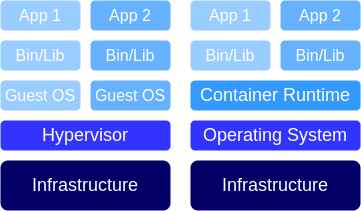
\includegraphics[width=\textwidth]{./images/vm_vs_container.png}
                \caption{Virtual Machine (left) and container (right) block model.\label{fig:differences}}
            \end{figure}
        \end{column}
    \end{columns}
\end{frame}

\begin{frame}
    \frametitle{Background Concepts}
    \framesubtitle{Checkpoint-Restore}

    \begin{columns}[t]
        \begin{column}{.65\textwidth}
            \textbf{\textcolor{blue}{Checkpoint-Restore in Userspace (CRIU):}}
            \begin{itemize}
                \item \textbf{\textcolor{blue}{Checkpointing}} is a technique that provides fault-tolerance for computing systems[6].
                \item \textbf{CRIU} is a tool to perform C/R from userspace, \textbf{\textcolor{blue}{transparently}} to the user [7,8].
                \item It is currently integrated in several container runtimes: we will use \texttt{runc} and \texttt{containerd}.
            \end{itemize}
            \textbf{\textcolor{blue}{Checkpointing Established TCP Connections:}}
            \begin{itemize}
                \item With the \texttt{TCP\_REPAIR} socket option added to kernel 3.5, it becomes possible to C/R established TCP sockets[9].
                \item Together with the support for restoring into existing namespaces, we can replicate the structure in Figure~\ref{fig:architecture}.
            \end{itemize}
        \end{column}
        \begin{column}{.3\textwidth}
            \vspace{-20pt}
            \begin{figure}[t!]
                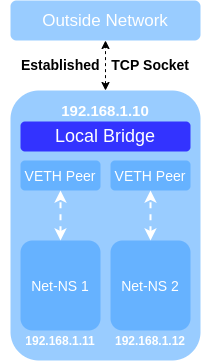
\includegraphics[width=.6\textwidth]{./images/tcp_arch.png}
                \caption{Architecture of the initial experiment.\label{fig:architecture}}
            \end{figure}
        \end{column}
    \end{columns}
\end{frame}

\begin{frame}
    \frametitle{Status of the Project}
    \framesubtitle{What we have}
    
    \textbf{\textcolor{blue}{(Not) Live Demo!}}
    \begin{center}
        \movie[width=.7\textwidth,height=.393\textwidth,showcontrols=true,poster,start=5s]{Click to play}{./videos/tcp_restore_inside_ns.mp4}
    \end{center}
\end{frame}

\begin{frame}
    \frametitle{Status of the Project}
    \framesubtitle{Problems Encoutnered and Moving Forward}

    \begin{columns}[t]
        \begin{column}{.45\textwidth}
            \textbf{\textcolor{blue}{Problems Encountered:}}
            \begin{enumerate}
                \item Lack of support in container runtimes.
                \item On-going project and very kernel-dependent.
                \item Lack of updated documentation, source as reference, what slows the development.
            \end{enumerate}
            \textbf{\textcolor{blue}{Alternatives:}}
            \begin{enumerate}
                \item Minimize the abstraction layers.
                \item On-going means active community.
                \item \texttt{Podman}, \texttt{runc}, \texttt{LXC} have it in their stack.
            \end{enumerate}
        \end{column}
        \begin{column}{.45\textwidth}
            \textbf{\textcolor{blue}{Moving forward:}}
            \begin{enumerate}
                \item Migrate server to a \emph{different} namespace (or machine) with the \emph{same} IP.
                \item Integrate with the \texttt{runc} runtime.
                \item Syncrhonize a C/R among a set of containers (or process).
                \begin{enumerate}
                    \item "Zero-Downtime" migration.\\[5pt]
                    \item Synchronous migration (close and re-establish connections).
                \end{enumerate}
            \end{enumerate}
        \end{column}
    \end{columns}
    
\end{frame}

\begin{frame}
    \frametitle{References}

    \textbf{\textcolor{blue}{Some links:}}

    \small

    \begin{enumerate}
        \item[[1]] \url{https://github.com/docker/cli/blob/master/experimental/checkpoint-restore.md}
        \item[[2]] \url{https://criu.org/Docker}
        \item[[3]] \url{http://man7.org/linux/man-pages/man7/cgroups.7.html}
        \item[[4]] \url{https://access.redhat.com/documentation/en-us/red_hat_enterprise_linux/6/html/resource_management_guide/ch01}
        \item[[5]] \url{http://man7.org/linux/man-pages/man7/namespaces.7.html}
        \item[[6]] \url{https://en.wikipedia.org/wiki/Application_checkpointing}
        \item[[7]] \url{https://en.wikipedia.org/wiki/CRIU}
        \item[[8]] \url{https://criu.org/Main_Page}
        \item[[9]] \url{https://criu.org/TCP_connection}
    \end{enumerate}

\end{frame}

\begin{frame}
    \frametitle{Questions \& Discussion}

    \begin{center}
        Thank you for your attention,\\[5pt]

        \Large
        \textbf{\textcolor{blue}{Observations, Doubts \& Suggestions Welcome}}\\[25pt]

        \normalsize
        Follow the development:\\ \url{https://github.com/live-containers/live-migration}\\[15pt]
        \url{carlos.segarra@estudiant.upc.edu}
    \end{center}
\end{frame}

\end{document}
